\documentclass[a4paper, 9pt, envcountsect]{beamer}

\vfuzz=50pt
\hfuzz=50pt

%generic=======================================================================

\usepackage[T3,T1]{fontenc}
\usepackage[english]{babel}
\usepackage{lmodern}
\usepackage{hyperref}
\usepackage{caption}
\usepackage{subcaption}

%math fonts====================================================================

\usepackage{bm}
\usepackage{dsfont}
\usepackage{stmaryrd}
\usepackage{amsfonts}

%algorithm=====================================================================
\usepackage{algorithm2e}

%images=========================================================================
\usepackage{wrapfig}
\usepackage{graphicx}
\graphicspath{{img/}}

%maths commands=================================================================
\usepackage{amsmath}
\usepackage{mathtools}

\newcommand{\matr}[1]{\mathbf{#1}}

\newtheorem{innercustomgeneric}{\customgenericname}
\providecommand{\customgenericname}{}
\newcommand{\newcustomtheorem}[2]{%
  \newenvironment{#1}[1]
  {%
   \renewcommand\customgenericname{#2}%
   \renewcommand\theinnercustomgeneric{##1}%
   \innercustomgeneric}
  {\endinnercustomgeneric}
}

\newcustomtheorem{thm}{Theorem}
\newcustomtheorem{dft}{Definition}

\DeclareMathOperator*{\argmin}{argmin}
\DeclareMathOperator*{\argmax}{argmax}

\let\llb\llbracket
\let\rrb\rrbracket

%other commands=================================================================
\let\ttsub\textsubscript
\let\ttsup\textsuperscript

\usepackage{tikz}

\newcommand{\bluecheck}{}%
\DeclareRobustCommand{\bluecheck}{%
  \tikz\fill[scale=0.4, color=blue]
  (0,.35) -- (.25,0) -- (1,.7) -- (.25,.15) -- cycle;%
}

\newcommand\Warning{%
 \makebox[1.4em][c]{%
 \makebox[0pt][c]{\raisebox{.1em}{!}}%
 \makebox[0pt][c]{\color{red}\Large$\bigtriangleup$}}
}%

%beamer config==================================================================
\usepackage{beamerthemesplit}
\usetheme{metropolis}
\setbeamertemplate{theorems}[numbered]
\metroset{sectionpage=simple, subsectionpage=simple}
\setbeamerfont{title}{size=\huge}

%title page=====================================================================

\title{DESeq2}
\institute[PhD student]{\textbf {MICS lab}\\ \textbf{Meta Prism}}
\author[Yoann Pradat]{
  \textbf{Yoann Pradat}\texorpdfstring{\\ \footnotesize{Supervised by P.H Cournède, D.  Gautheret}}{}
}
\titlegraphic{%
  \begin{picture}(0,0)
    \put(150,-195){{
\includegraphics[width=1.5cm]{mics_logo.png}}}
    \put(225,-200){{
\includegraphics[width=2.0cm]{prism_logo.png}}}
  \end{picture}}
\date{\today}

%begin=========================================================================

\begin{document}
\frame{\maketitle}

{
\metroset{sectionpage=none}
\section*{Sommaire}
\frame{\tableofcontents}
}


{
\metroset{sectionpage=none}
\section{Introduction}

\frame{\frametitle{Introduction}
  {\small
  \underline{1\ttsup{st} paper}: Anders S, Huber W: \textbf{Differential expression analysis for sequence count data}.  
  \textit{Genome Biol} 2010, 11:106. ($\sim$ 11k citations, \texttt{DESeq} R package)

  \underline{2\ttsup{nd} paper}: Love, M.I., Huber, W., Anders, S. \textbf{Moderated estimation of fold change and 
  dispersion for RNA-seq data with DESeq2}. \textit{Genome Biol} 2014, 15:550. ($\sim$ 20k citations, \texttt{DESeq2} R 
  package)

  \underline{Vignette}: \url{https://www.bioconductor.org/packages/devel/bioc/vignettes/DESeq2/inst/doc/DESeq2.html}

  \medbreak

  \underline{Affiliations:} 
  \begin{itemize}
    \item Michael I. Love -> Dana Farber Institute, Boston.
    \item Wolfgang Huber, Simon Anders -> EMBL, Heidelberg.
  \end{itemize}
  }
}
}

\section{DESeq2 Methods}

\subsection{The model(s)}

\frame{\frametitle{Counting data with Negative Binomial}
  \underline{Notations}
  \begin{itemize}
    \item $i=1,\ldots,n$ denote count variables (genes).
    \item $j=1,\ldots,m$ denote individuals.
    \item $\mathrm{K_{ij}}$ count of var $i$ in indiv $j$, $\matr{K} = \matr{K}_{1:n, 1:m}$ count matrix.
    \item $\matr{X}_j$ covariates of indiv $j$, $\matr{X} = \matr{X}_{1:m, 1:p}$ design matrix.
  \end{itemize}
  \pause
  The negative binomial $\mathrm{NegBin}(r,p)$ counts the number of failures before $r$ successes of proba $p$.
  \begin{equation}
    p_{\mathrm{NegBin}(r, p)}(k) = \frac{(k+r-1)!}{k!(n-1)!} p^r (1-p)^k
  \end{equation}
  Other formulation with mean and dispersion
  \begin{equation}
    p_{\mathrm{NegBin}(\mu, \alpha)}(k) = \frac{\Gamma(k+\alpha^{-1})}{\Gamma(\alpha^{-1})k!} \left(\frac{1}{1 + 
    \alpha\mu}\right)^{\alpha^{-1}} \left(\frac{\mu}{\alpha^{-1} + \mu}\right)^{k}
  \end{equation}
}

\frame{\frametitle{The model(s)}
  \texttt{DESeq2} models the counts $\mathrm{K_{ij}}$ distribution conditionally to $\mathrm{X_j}$ as
  \begin{equation}
    \boxed{\mathds{P}_{\mathrm{K_{ij}|X_{j}}=x_j} = \mathrm{NegBin}(\mu_{ij}, \alpha_i)}
  \end{equation}
  with a logarithmic link
  \begin{equation*}
    \log(\mu_{ij}) = x_j^\top \beta_i
  \end{equation*}
  or rather, in order to account for indiv-specific size factors,
  \begin{equation}
    \log\left(\frac{\mu_{ij}}{s_j}\right) = x_j^\top \beta_i
  \end{equation}
  \pause

  \underline{Model fitting}: Find \textbf{estimators}
  \begin{enumerate}
    \item $\hat{s}_{1:m}$ (size factors)
    \item $\hat{\alpha}_{1:n}$ (dispersions)
    \item $\hat{\beta}_{1:n}$ (log fold changes)
  \end{enumerate}
}

\subsection{Size factors estimators}

\frame{\frametitle{Size factors estimators}
  \underline{Simple estimator} Let 
  \begin{equation}
    K^R_i = \left(\prod_{j=1}^m K_{ij} \right)^\frac{1}{m}
  \end{equation}
  Then,
  \begin{equation}
    \hat{s}_j = \underset{K^R_i \neq 0}{\text{median}} \left\{ \frac{K_{ij}}{K^R_i} \right\}
  \end{equation}
  \pause
  \underline{Model fitting}: Find \textbf{estimators}
  \begin{enumerate}
    \item $\hat{s}_{1:m}$ (size factors) \bluecheck
    \item $\hat{\alpha}_{1:n}$ (dispersions)
    \item $\hat{\beta}_{1:n}$ (log fold changes)
  \end{enumerate}
}


\subsection{Dispersion estimators}

\frame{\frametitle{Dispersion estimators via prior}
  Instead of estimating directly the dispersions $\alpha_i$, they have their own distribution (prior) that is to be 
  fitted to the data (posterior).

  \begin{equation}
    \mathds{P}_{\alpha_i} = \mathcal{LN}\left(\alpha_\mathrm{tr}(\bar{\mu}_i), \sigma_d^2\right)
  \end{equation}
  with $\alpha_\mathrm{tr}(\bar{\mu}) = a_0 + \frac{a_1}{\bar{\mu}}$, $\bar{\mu}_i = \frac{1}{m} \sum_{j=1}^m 
  \frac{K_{ij}}{s_j}$.

  \hspace{10pt}

  \pause
  \underline{However}, the dispersions are not observed. \underline{To remedy to this}, authors derive initial values of 
  dispersion $\alpha_{i}^\mathrm{gw}$ that are used to estimate $\alpha_\mathrm{tr}$ and $\sigma_d^2$.

  \underline{Dispersion fitting}: Find \textbf{estimators}
  \begin{enumerate}
    \item $\alpha_i^\mathrm{gw}$ (gene wise initial estimates)
    \item $\hat{\alpha}_\mathrm{tr}, \hat{\sigma}_{d}^2$ (prior dispersions)
    \item $\alpha_i^\mathrm{MAP}$ (MAP estimators)
  \end{enumerate}

  \underline{Remark}: All genes with 0 counts are excluded from further analyses.
}

\frame{\frametitle{The model matrix $\matr{X}$}
  \Warning $\matr{X}$ is the \textbf{model matrix} and it is obtained from the \texttt{DESeq2DataSet} object using the 
  formula \texttt{colData(dds)} and \texttt{design(dds)}.

  Examples with \texttt{colData(dds) = $\left[\text{condition}(0,0,1) \ \text{type}(A,B,C) \right]$}
  \begin{enumerate}
    \item $\texttt{design} = \sim\text{condition}$,
      \begin{equation}
        \matr{X} = \begin{bmatrix} 
          \text{intercept} & \text{condition} \\
          \text{1}         & \text{0}         \\
          \text{1}         & \text{0}         \\
          \text{1}         & \text{1}         \\
        \end{bmatrix}
      \end{equation}
      For this $\matr{X}$, the model for $\hat{\mu}_i$ \textbf{is linear} (except if weights are used).
    \pause
    \item $\texttt{design} = \sim\text{condition} + \text{type} $,
      \begin{equation}
        \matr{X} = \begin{bmatrix}
          \text{intercept} & \text{condition} & \text{type} \\
          \text{1}         & \text{0}         & A           \\
          \text{1}         & \text{0}         & B           \\
          \text{1}         & \text{1}         & C           \\
        \end{bmatrix}
      \end{equation}
      For this $\matr{X}$, the model for $\hat{\mu}_i$ \textbf{is the NegBin GLM}.
  \end{enumerate}
}

\frame{\frametitle{Initial gene-wise dispersion estimators}
  Initial estimation of gene-wise dispersions as a minimum
  \begin{equation}
    \alpha_{i}^\mathrm{init} = \min (\alpha_i^\mathrm{rough}, \alpha_i^\mathrm{moment})
  \end{equation}
  with 
  \begin{align*}
    \alpha_i^\mathrm{rough} &= \frac{1}{m-p} \sum_{j=1}^m  \frac{(\tilde{K}_{i,j} - \tilde{\mu}_{i,j})^2 - 
      \tilde{\mu}_{i,j}^2}{\tilde{\mu}_{i, j}^2}, && \smash{
        \left\{\begin{array}{@{}l@{}}
            \tilde{\mu}_{i,1:m} = \matr{X} \hat{\tilde{\beta}}_{i} \ (\text{\small{linear for all $\matr{X}$}}) \\ 
            [\jot]
          \hat{\tilde{\beta}}_{i} = \argmin_{\beta} \| \matr{\widetilde{K}_{i,1:m}} - \matr{X} \beta \|^2_2
        \end{array}\right.
      }  \\
    \alpha_i^\mathrm{moment} &= \frac{\sigma^2(\matr{\widetilde{K}_{i,1:m}}) - \mu(\matr{\widetilde{K}_{i,1:m}}) 
    \mu(\hat{\matr{S}}_{1:m}^{-1})}{\mu(\matr{\widetilde{K}_{i,1:m}})^2}
  \end{align*}
  \pause
  \texttt{DESeq2} restricts by default the dispersion estimates as follows
  \begin{equation}
    \alpha_{i}^\mathrm{init} = \min(\max(10^{-8}, \alpha_i^\mathrm{init}),\max(10,m))
  \end{equation}
}

\frame[shrink]{\frametitle{Iterative MLE gene-wise dispersion estimators}
  \vspace{10pt}
  \begin{algorithm}[H]
    \KwResult{$\alpha_i^\mathrm{gw} = \alpha_i^{(T)}$}
    initialization $\alpha_i^{(0)} = \alpha_i^\mathrm{init}$\;
    \For{$t=1,\ldots,T$}
      {
        \begin{equation*}
            \hat{\mu}^{(t)}_{i, 1:m} =
              \begin{dcases}
                \matr{\hat{S}_{1:m}} \odot \tilde{\mu}_{i, 1:m} & \text{if linear model} \\
                \argmax_{\mu_{1:m}} \prod_{j=1}^m p_\mathrm{NegBin(\mu_j, \hat{\alpha}_i^{(t-1)})}(K_{i,j}) & 
                \text{otherwise}
              \end{dcases};
        \end{equation*}\
        \begin{equation*}
            \hat{\alpha}^{(t)}_{i} =
              \begin{dcases}
                \argmax_{\alpha} \frac{1}{\sqrt{\det(\matr{X^\top W X})}} \prod_{j=1}^m 
                p_\mathrm{NegBin(\hat{\mu}_{i,j}^{(t)}, \alpha)}(K_{i,j}) & \text{if \texttt{DESeq2} type} \\
                \texttt{\small{overdispersion}}(y=\matr{K_{i,1:m}}, \mu = \hat{\mu}^{(t)}_{i,1:m}, \matr{X=X})
                                  & \text{if \texttt{glmGamPoi} type}
              \end{dcases};
        \end{equation*}\
      }
    if estimator $\alpha_i^{(T)}$ did not converge and $\alpha_i^{(T)} > 10^{-7}$, then
    \begin{equation*}
      \alpha^\mathrm{gw}_{i} = \argmax_{\alpha} \frac{1}{\sqrt{\det(\matr{X^\top W X})}} \prod_{j=1}^m 
      p_\mathrm{NegBin(\hat{\mu}_j^{(T)}, \alpha)}(K_{i,j}) \quad \text{on a grid (\texttt{fitDispGrid})}
    \end{equation*}
  \end{algorithm}
}

\frame[shrink]{\frametitle{Fit the dispersion prior mean}
  \underline{Dispersion fitting}: Find \textbf{estimators}
  \begin{enumerate}
    \item $\alpha_i^\mathrm{gw}$ (gene wise initial estimates) \bluecheck
    \item $\hat{\alpha}_\mathrm{tr}, \hat{\sigma}_{d}^2$ (prior dispersions)
    \item $\alpha_i^\mathrm{MAP}$ (MAP estimators)
  \end{enumerate}
  \begin{enumerate}
    \item \textbf{Trend}
      \begin{minipage}{.4\textwidth}%
      The prior model is
      \begin{equation*}
        \mathds{P}_{\alpha} = \mathcal{LN}\left(a_0  + \frac{a_1}{\bar{\mu}}, \sigma^2_d\right)
      \end{equation*}
      DESeq2 uses
    \end{minipage}%
    \begin{minipage}{.6\textwidth}%
      \begin{figure}
        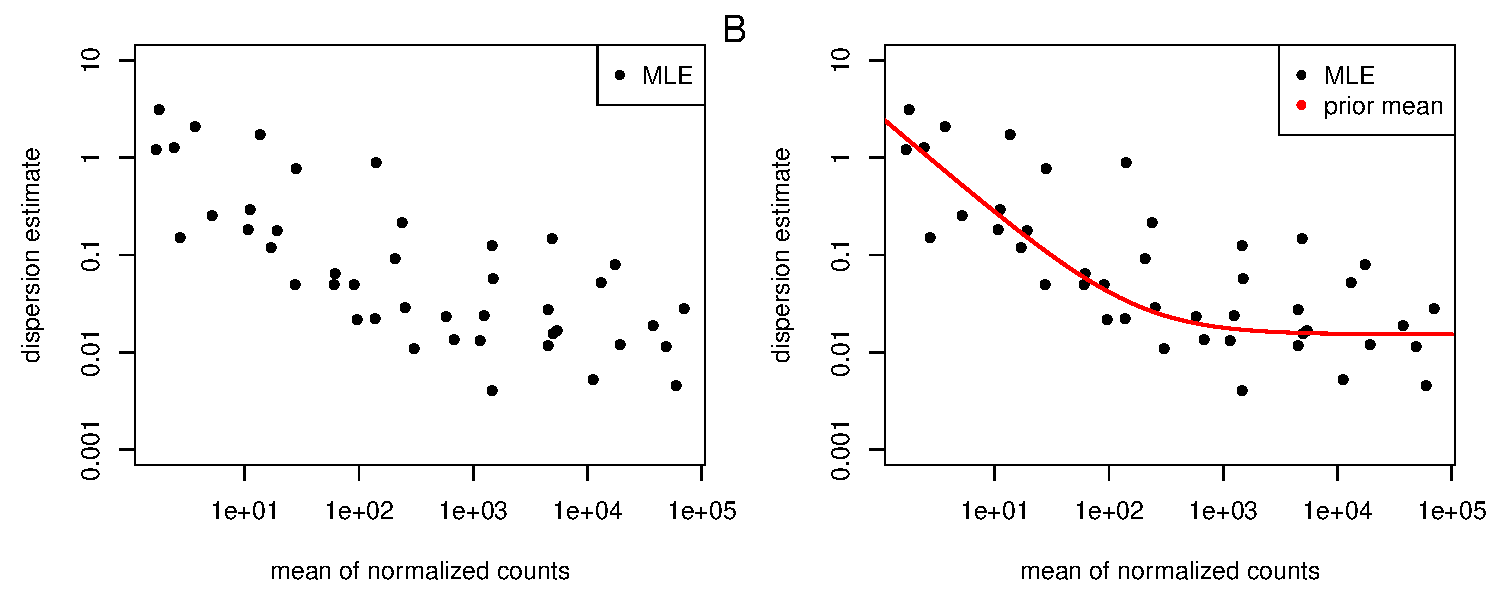
\includegraphics[width=1.5\textwidth]{plotDispShrink_gw_and_trend.pdf}
      \end{figure}
    \end{minipage}
    \begin{equation*}
      \begin{dcases}
        \text{10 iterations of} \quad \mathds{P}_{\alpha|\bar{\mu}=\bar{\mu}} = \Gamma\left(a_0 + 
          \frac{a_1}{\bar{\mu}}, \phi\right) & \text{if type=\texttt{parametric} \quad with $a_0^{(0)} = 0.1, 
        a_1^{(0)} = 1$} \\
          \texttt{locfit} & \text{if type=\texttt{locfit} or failed \texttt{parametric}} \\
        \texttt{loc\_median\_fit} & \text{if type=\texttt{glmGamPois}}
    \end{dcases}
    \end{equation*}
    \Warning $\Gamma$ regression ignores points with log residual outside $[10^{-4}, 15]$.
    \pause
    \item\textbf{Variance}
      \begin{equation*}
        \widehat{\sigma_d^2} = \max \{ s^2_\mathrm{lr} - \psi_1(\frac{m-p}{2}), 0.25\}
      \end{equation*}
      with $s^2_\mathrm{lr}$ a robust estimator
      \begin{equation*}
        s^2_\mathrm{lr} = \underset{i}{\text{mad}} \{\log (\alpha_i^\mathrm{gw}) - \log 
        \alpha_\mathrm{tr}(\bar{\mu_i})\}
      \end{equation*}
  \end{enumerate}
}

\frame[shrink]{\frametitle{MAP dispersion estimators}
  \underline{Dispersion fitting}: Find \textbf{estimators}
  \begin{enumerate}
    \item $\alpha_i^\mathrm{gw}$ (gene wise initial estimates) \bluecheck
    \item $\hat{\alpha}_\mathrm{tr}, \hat{\sigma}_{d}^2$ (prior dispersions) \bluecheck
    \item $\alpha_i^\mathrm{MAP}$ (MAP estimators)
  \end{enumerate}
  \pause
  \begin{minipage}{.4\textwidth}%
    \begin{enumerate}
      \item $\alpha_i^\mathrm{gw}$ is an \textbf{outlier} if
        \begin{equation*}
          \log (\alpha_i^\mathrm{gw}) - \log \hat{\alpha}_\mathrm{tr}(\bar{\mu_i}) > 2 s^2_\mathrm{lr}
        \end{equation*}
        Then, $ \alpha_i^\mathrm{final} = \alpha_i^\mathrm{gw}$.
      \item Otherwise,
    \end{enumerate}
  \end{minipage}%
  \begin{minipage}{.6\textwidth}%
    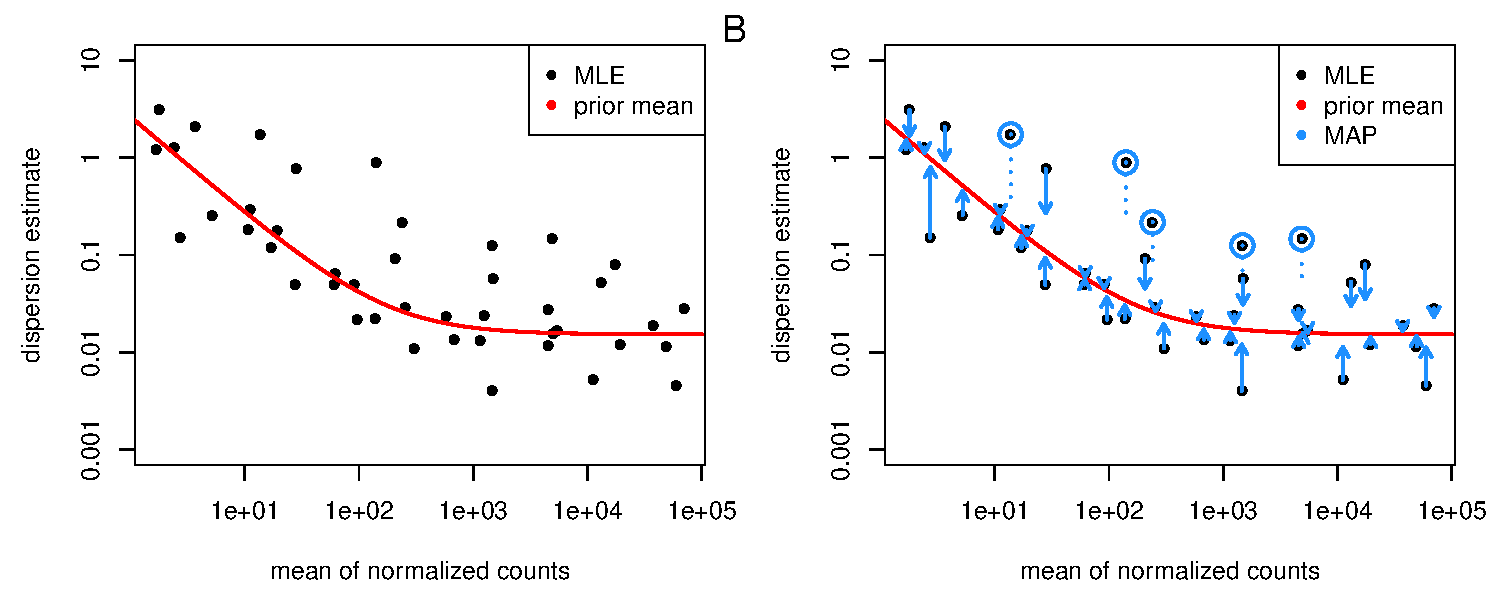
\includegraphics[width=1.25\textwidth]{plotDispShrink_gw_trend_and_MAP.pdf}
  \end{minipage}
  \begin{equation}
    \alpha_i^{\mathrm{final}} = \argmax_{\alpha} p_{\alpha_i|\mathrm{K_{i,1:m}}=\matr{k_{i,1:m}}}(\alpha) \propto 
    \prod_{j=1}^m p_{\mathrm{K_{i,j}}|\alpha_i=\alpha}(k_{ij}) p_{\alpha_i}(\alpha)
  \end{equation}

  \underline{Model fitting}: Find \textbf{estimators}
  \begin{enumerate}
    \item $\hat{s}_{1:m}$ (size factors) \bluecheck
    \item $\hat{\alpha}_{1:n}$ (dispersions) \bluecheck
    \item $\hat{\beta}_{1:n}$ (log fold changes)
  \end{enumerate}
}

\subsection{LFC estimators}

\frame{\frametitle{LFC model and estimation}
  \underline{Reminder}:
  \begin{equation}
    \boxed{\mathds{P}_{\mathrm{K_{ij}|X_{j}}=x_j} = \mathrm{NegBin}(s_je^{x_j^\top \beta_i}, \alpha_i)}
  \end{equation}

  As for dispersions, author set a prior on each $\beta_{i, r}$,
  \begin{equation}
    \mathds{P}_{\beta_{i,r}} = \mathcal{N}\left(0, \sigma^2_r\right)
  \end{equation}

  \underline{LFC fitting}: Find \textbf{estimators}
  \begin{enumerate}
    \item $\beta_i^\mathrm{MLE}$ (initial estimates)
    \item $\hat{\sigma}_{r}^2$ (prior fitting)
    \item $\beta_i^\mathrm{MAP}$ (MAP estimators)
  \end{enumerate}
}

\frame{\frametitle{Prior fitting}
  \begin{enumerate}
    \item Initial estimation of gene-wise LFC as a minimum
      \begin{equation}
        \beta_{i}^\mathrm{MLE} = \argmax_\beta \prod_{j=1}^m p_\mathrm{NegBin(\hat{s_j}e^{\beta^T x_j}, 
        \hat{\alpha}_i^{final})}(K_{i,j})
      \end{equation}
    \item Variance estimator robust against LFC outliers
      \begin{equation*}
        \hat{\sigma}_r  = \frac{Q_{|\beta_r^\mathrm{MLE}|}(1-p)}{Q_N(1-p/2)}
      \end{equation*}
      $p$ is set to 0.05 by default
  \end{enumerate}
  \underline{LFC fitting}: Find \textbf{estimators}
  \begin{enumerate}
    \item $\beta_i^\mathrm{MLE}$ (initial estimates) \bluecheck
    \item $\hat{\sigma}_{r}^2$ (prior fitting) \bluecheck
    \item $\beta_i^\mathrm{MAP}$ (MAP estimators)
  \end{enumerate}
}

\frame{\frametitle{Posterior fitting}
  \begin{enumerate}
    \item \textbf{LFC final estimator}
  \begin{align*}
    \beta_{i, 1:p}^{\mathrm{final}} &= \argmax_{\beta} \frac{1}{\sqrt{\det(\matr{X^\top W X})}} 
    p_{\beta_i|\mathrm{K_{i,1:m}}=\matr{k_{i,1:m}}}(\beta) \\
                                    &\propto \frac{1}{\sqrt{\det(\matr{X^\top W X})}} \prod_{j=1}^m 
                                    p_{\mathrm{K_{i,j}}|\beta_i=\beta}(k_{ij}) p_{\beta_i}(\beta)
  \end{align*}
  i.e
  \begin{equation*}
    \beta_{i,1:p}^{\mathrm{final}} = \argmax_{\beta} \sum_{j=1}^m \log p_{\mathrm{NegBin}(\mu_j(\beta), 
    {\color{red}\hat{\alpha}_i})}(K_{i,j}) - \frac{1}{2} \log \det (\matr{X^\top W X}) - \sum_{r=1}^p 
    \frac{\beta_r^2}{2\sigma_r^2}
  \end{equation*}

    \item \textbf{Estimator of covariance LFC estimator}
    Also estimate the covariance matrix $\Sigma_{i} = \widehat{\mathrm{Cov}}\left(\beta_i^\mathrm{final}\right)$ for the 
    tests.
  \end{enumerate}
}

\frame[shrink]{\frametitle{Other LFCs priors}
  Authors observed "\textit{normal prior can sometimes produce too strong of a shrinkage}". From v1.18, additional 
  priors may be used
  \begin{enumerate}
    \begin{minipage}{.5\textwidth}%
    \item \texttt{apeglm} adaptive t prior from the \texttt{apeglm} package (Zhu, Ibrahim and Love, Bioinformatics 
      2018). The prior is 
      \begin{equation}
        \mathds{P}_{\beta_{ir}} = \mathrm{Cauchy}(0, S_r)
      \end{equation}
    \end{minipage}%
    \begin{minipage}{.5\textwidth}%
      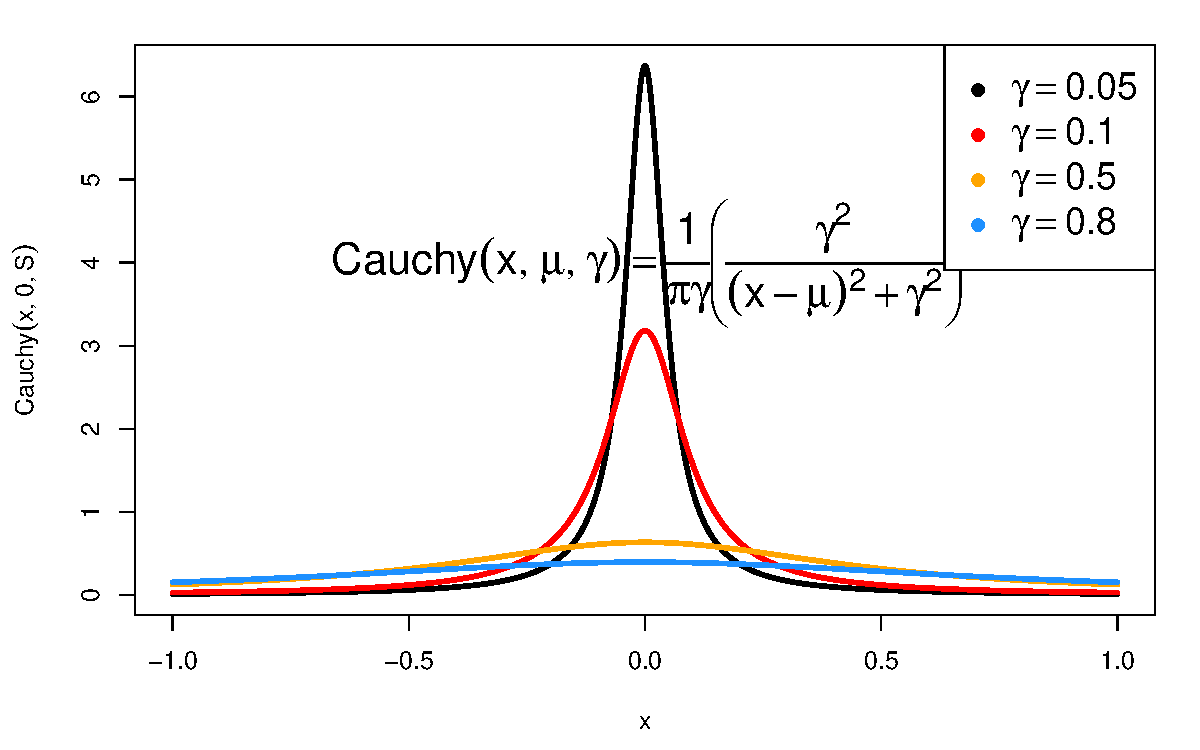
\includegraphics[width=\textwidth]{plotCauchy.pdf}
    \end{minipage}
    \item \texttt{ashr}  from \texttt{ashr} package (Stephens, Biostatistics 2016). New approach to bridge the gap 
      between \textbf{FDR} and \textbf{estimation} using "local false sign rate". Assuming there are effect and SE 
      estimates, $\hat{\beta}_{i,1:p}$ and $\hat{S}_{i,1:p}$, ashr computes
      \begin{equation*}
        p_{\beta_{i}|\hat{\beta}_i,\hat{S}_i}(\beta) \propto p_{\hat{\beta}_i|\beta_i, \hat{S}_i}(\hat{\beta}_i) 
        p_{\beta_i|\hat{S}_i}(\beta)
      \end{equation*}
      with
      \begin{equation*}
        p_{\hat{\beta}_i|\beta_i, \hat{S}_i}(\beta) = \prod_{r=1}^p \mathcal{N}(\beta_{r}|\beta_{i,r}, \hat{S}_{i,r}^2) 
        \quad, \mathds{P}_{\beta_i|\hat{S}_i} = \pi_{0,i} \delta_0 + \sum_{k=1}^K \pi_{k,i} \mathcal{N}(0, 
        \sigma_{i,k}^2).
      \end{equation*}
  \end{enumerate}
}

\subsection{LFC testing}

\frame{\frametitle{Wald testing}
  \begin{enumerate}
    \item Using the LFC estimator and the estimation of the covariance of this LFC estimator, one may form Wald 
      statistics
    \begin{equation}
      \frac{\beta_{i,r}^\mathrm{final}}{\sqrt{\Sigma_{i,rr}}}
    \end{equation}
    \item \textbf{Only} the $p$-values for the genes that \textbf{individually pass the independent filtering step} are 
      adjusted using BH procedure. \\

      \underline{Independent filtering}: threshold on
      \begin{equation*}
        \bar{K}_i = \frac{1}{m} \sum_{j=1}^m \tilde{K}_{ij}
      \end{equation*}

      \underline{Ref}: \small{Wolfgang Huber: Independent filtering increases detection power for high-throughput 
      experiments. PNAS (2010), \url{http://dx.doi.org/10.1073/pnas.0914005107}}
  \end{enumerate}
}

\section{Questions}

\end{document}
